\begin{figure}[ht]
\centering
% Thesis-wide categorical color palette
% Usage: % Thesis-wide categorical color palette
% Usage: % Thesis-wide categorical color palette
% Usage: \input{figures/palette} in any figure file
%
% Muted primary colors -- print-friendly, visually distinct.
% Inspired by Cooper Union's red/blue primaries, softened for
% academic figures. Use palA-palC for data series in scatter
% plots, line charts, bar charts, etc.

\definecolor{palA}{HTML}{1F77B4}   % Tableau blue
\definecolor{palB}{HTML}{D62728}   % Tableau red
\definecolor{palC}{HTML}{2CA02C}   % Tableau green
 in any figure file
%
% Muted primary colors -- print-friendly, visually distinct.
% Inspired by Cooper Union's red/blue primaries, softened for
% academic figures. Use palA-palC for data series in scatter
% plots, line charts, bar charts, etc.

\definecolor{palA}{HTML}{1F77B4}   % Tableau blue
\definecolor{palB}{HTML}{D62728}   % Tableau red
\definecolor{palC}{HTML}{2CA02C}   % Tableau green
 in any figure file
%
% Muted primary colors -- print-friendly, visually distinct.
% Inspired by Cooper Union's red/blue primaries, softened for
% academic figures. Use palA-palC for data series in scatter
% plots, line charts, bar charts, etc.

\definecolor{palA}{HTML}{1F77B4}   % Tableau blue
\definecolor{palB}{HTML}{D62728}   % Tableau red
\definecolor{palC}{HTML}{2CA02C}   % Tableau green


%% Panel (a): The transition on the grid
\begin{subfigure}[t]{0.42\textwidth}
\centering
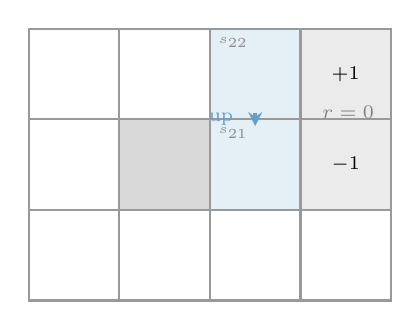
\begin{tikzpicture}[
    cell/.style={minimum size=1.15cm, draw=black!40, thick},
    wall/.style={cell, fill=black!15},
    terminal/.style={cell, fill=black!8},
    highlight/.style={cell, fill=palA!12},
    arr/.style={->, thick, >=stealth},
    plabel/.style={font=\scriptsize\bfseries},
    slabel/.style={font=\tiny, text=black!45, anchor=north west},
]
\def\s{1.15}

% Full 4x3 grid
% Row 0
\node[cell] (c00) at (0, 0) {};
\node[cell] (c10) at (\s, 0) {};
\node[cell] (c20) at (2*\s, 0) {};
\node[cell] (c30) at (3*\s, 0) {};
% Row 1
\node[cell] (c01) at (0, \s) {};
\node[wall] (c11) at (\s, \s) {};
\node[highlight] (c21) at (2*\s, \s) {};
\node[terminal] (c31) at (3*\s, \s) {};
% Row 2
\node[cell] (c02) at (0, 2*\s) {};
\node[cell] (c12) at (\s, 2*\s) {};
\node[highlight] (c22) at (2*\s, 2*\s) {};
\node[terminal] (c32) at (3*\s, 2*\s) {};

% State labels
\node[slabel] at (c21.north west) {$s_{21}$};
\node[slabel] at (c22.north west) {$s_{22}$};

% Terminal labels
\node[plabel] at (c31) {$-1$};
\node[plabel] at (c32) {$+1$};

% Action arrow
\draw[arr, palA!70, very thick]
    ([yshift=2pt]c21.north) -- ([yshift=-2pt]c22.south)
    node[midway, left=4pt, font=\scriptsize, text=palA!70]
    {up};

% Reward annotation
\node[font=\scriptsize, text=black!50, right=4pt]
    at ([yshift=2pt]c21.north east) {$r = 0$};

\end{tikzpicture}
\subcaption{The agent in $s_{21}$ moves up to $s_{22}$,
  receiving reward $r = 0$.}
\label{fig:td-update-transition}
\end{subfigure}
\hfill
%% Panel (b): The bootstrap update
\begin{subfigure}[t]{0.52\textwidth}
\centering
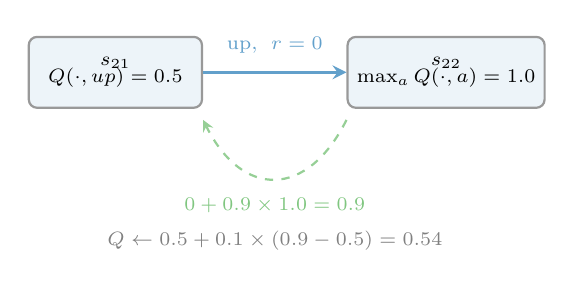
\begin{tikzpicture}[
    state/.style={draw=black!40, thick, rounded corners=3pt,
                  minimum width=2.2cm, minimum height=0.9cm,
                  font=\scriptsize, align=center, fill=palA!8},
    arr/.style={->, thick, >=stealth},
    lbl/.style={font=\scriptsize, text=black!55},
]

% State boxes (horizontal layout)
\node[state] (s21) at (0, 0)
    {$s_{21}$\\[-2pt] $Q(\cdot, \text{up}) = 0.5$};

\node[state] (s22) at (4.2, 0)
    {$s_{22}$\\[-2pt] $\max_a Q(\cdot, a) = 1.0$};

% Forward arrow: action + reward
\draw[arr, palA!70, very thick]
    (s21.east) -- (s22.west)
    node[midway, above=3pt, font=\scriptsize, text=palA!70]
    {up,\; $r = 0$};

% Bootstrap arrow (curved, below)
\draw[arr, palC!50, dashed, thick]
    ([yshift=-4pt]s22.south west)
    .. controls +(-0.5, -1.0) and +(0.5, -1.0) ..
    ([yshift=-4pt]s21.south east)
    node[midway, below=3pt, font=\scriptsize, text=palC!60]
    {$0 + 0.9 \times 1.0 = 0.9$}
    node[midway, below=15pt, font=\scriptsize, text=black!50]
    {$Q \leftarrow 0.5 + 0.1 \times (0.9 - 0.5) = 0.54$};

\end{tikzpicture}
\subcaption{The estimate at $s_{22}$ bootstraps back.
  The target updates $Q(s_{21}, \text{up})$ toward $0.9$.}
\label{fig:td-update-bootstrap}
\end{subfigure}

\caption{One Q-learning update step in the grid-world.}
\label{fig:td-update}
\end{figure}
